% SPDX-FileCopyrightText: 2026 Hasan Melih Akbulut
% SPDX-License-Identifier: CC-BY-4.0

\chapter{Introduction}
\label{ch:intro}

\section{The part}
\label{sec:intro-part}

This document describes a fault-tolerant system-on-chip for on-board AI
inference in small-satellite missions~\cite{naoukin2023}, implemented on
a 130\,nm technology with an open-source RTL-to-GDS flow
(\code{README.md}; \dcite{00-index}{section 1}). Its architecture class
follows the Frontgrade Gaisler GR801~\cite{gr801} as published in that
device's April 2026 product brief --- a RISC-V management processor, an
event-driven neuromorphic inference engine, on-chip SRAM and a set of
spacecraft interfaces --- retargeted from 28\,nm FDSOI to 130\,nm at a scale an open
PDK and one person can carry
(\code{docs/00-reference-brief.md}; \dcite{01}{section 2}).

What exists in the repository is two designs and a corpus of
measurements about them. The first design is a frozen accelerator slice
submitted to a multi-project shuttle and pinned by hash
(\dcite{34}{section 1}). The second is a management subsystem begun
after that freeze and kept strictly separate from it: an Ibex RV32IMC
core in its \code{small-pmp} configuration --- PMP, no lockstep --- on a
fabric that speaks Ibex's own protocol internally and real AMBA 3 APB at
the peripheral boundary, with a RISC-V CLINT, a GRLIB-style general
purpose timer, a watchdog that escalates through a non-maskable
interrupt to a system reset to an external pin, a console UART, a 16-pin
GPIO port, a register-mode QSPI flash controller with two chip selects,
a boot ROM that loads and verifies an image out of flash, and the frozen
accelerator instantiated inside it over the same four serial pins the
die will have (\code{docs/38}, \code{docs/39}, \code{docs/40},
\code{docs/41}, \code{docs/51}, \code{docs/65}, \code{docs/66}, \code{docs/68}).
That subsystem has been synthesised, placed and routed whole, most
recently as an eight-macro layout carrying the boot ROM's
error-correcting check macros, with zero detailed-routing violations, a
unique Netgen LVS match, and all four geometric deck families run on it
(\dcite{67}{section 11}).

\begin{figure}[tbp]
  \centering
  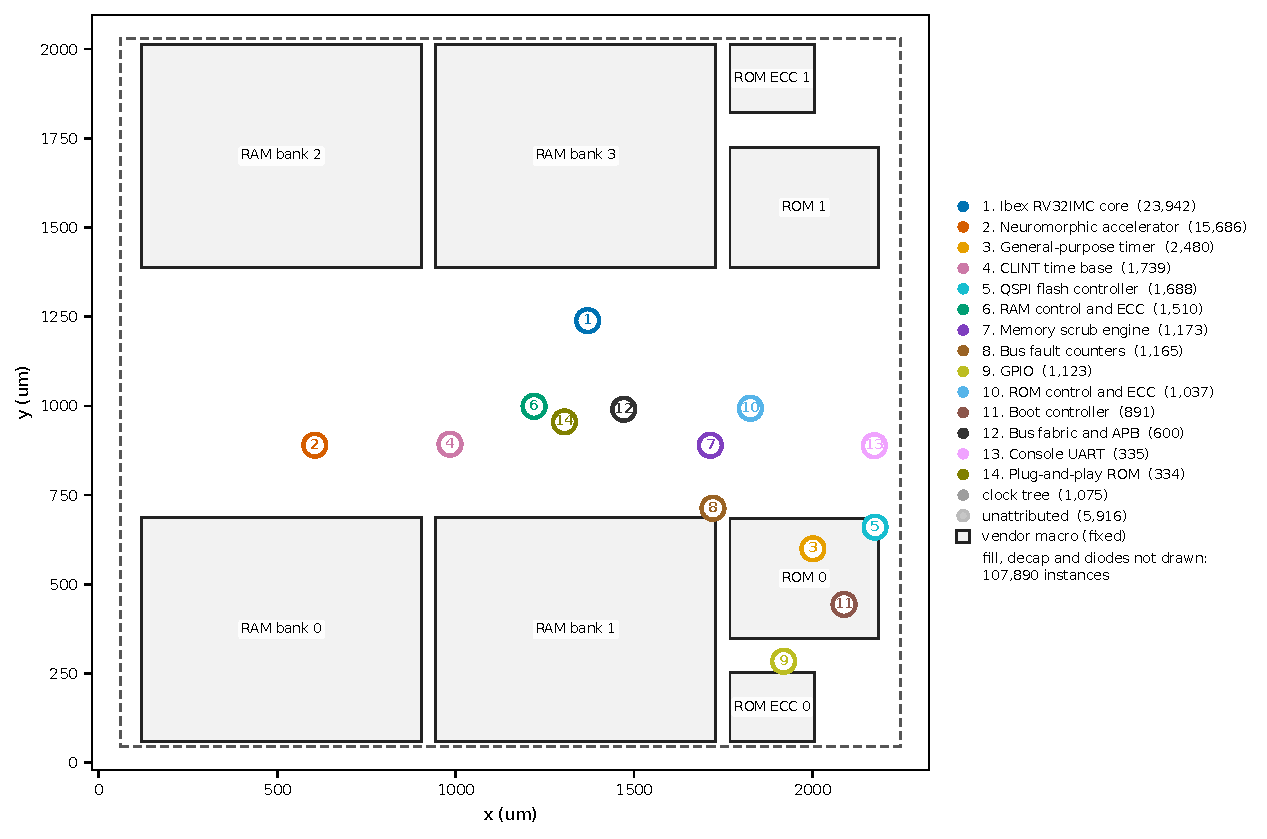
\includegraphics[width=\linewidth]{figures/layout_blocks.pdf}
  \caption[The system-on-chip, as placed]{The whole die, with every
  standard cell coloured by the block it belongs to and the eight vendor
  memory macros drawn and labelled, read out of run
  \code{s83romecc5}'s own DEF and netlist --- the eight-macro layout of
  \dcite{67}{section 11}. The die is
  2306.40 by 2075.22\,\si{\micro\metre}, that is
  \qty{4786287.408}{\micro\metre\squared} (\dcite{59}{section 3.1}). Apart
  from the eight macros, which are fixed, nothing here was told where to
  go: the clusters are the placer's, not the designer's. Only about
  7{,}700 of the die's instances still carry a hierarchical name after
  synthesis --- the generator's docstring figure, beside a comment in
  the same file counting 1{,}140 instance names with a dot in them ---
  so the block attribution is made by connectivity --- nets
  keep their hierarchical names, each anonymous cell takes the block
  most of its pins' nets vote for, and two rounds of neighbour
  propagation follow --- and the
  \qty{9.75}{\percent} that never resolves is drawn grey and counted in
  the legend rather than hidden
  (\code{make\_layout\_figures.py} and
  \code{layout\_attribution.json}, both in \code{thesis/figures/}).
  Read the per-block
  counts as an attribution with that error bar on it, not as a census.}
  \label{fig:intro-blocks}
\end{figure}

\Cref{fig:intro-blocks} is the part. It carries 168{,}592 instances, of
which eight are the vendor SRAM macros and 168{,}584 are standard cells;
the two largest attributed blocks are the Ibex core at 23{,}942 cells
and the accelerator at 15{,}686, and 107{,}890 of the total are fill,
decap and diode cells that belong to no block and are not drawn
(\code{thesis/figures/layout\_attribution.json}). Those per-block
figures are the output of the attribution method described in the
caption, and the method's own 9.75\,\% unattributed remainder is the
error bar that travels with every one of them. A reader who wants a
census of a block should take it from that block's synthesis record, not
from this picture; what the picture is for is the question
``where is the processor, where is the memory'', which no table answers
as quickly.

\section{What this is not}
\label{sec:intro-not}

Four negatives bound everything that follows, and each is a matter of
record rather than of modesty.

\textbf{There is no silicon of this system-on-chip, and no tape-out of
it.} Nothing in the repository has been fabricated
(\dcite{00-index}{section 2.2}). The one design that has been submitted
anywhere is the pilot of \Cref{sec:intro-two-parts}, and even there the
shuttle slot was still an open owner action at the time of writing, with
the close at 2026-09-21 20:00 UTC (\code{ROADMAP.md} section 4 item 1).
A full-SoC run is gated on two things the pilot cannot settle: the SRAM
macro sign-off blocker of \Cref{sec:intro-pdk}, which is upstream, and a
timing constraint the layout does not meet (\code{ROADMAP.md} section 1).

\textbf{No clock frequency is claimed for this design.} This is a rule,
not an omission, and \Cref{sec:intro-rules} gives its three reasons. The
consequence for the reader is that every timing result in this document
is reported as a period, a slack and a corner name, in the words the
tool used: the system-on-chip is constrained at a 20\,ns period and
misses it by \qty{-3.2029}{\nano\second} on 2{,}003 endpoints at the
\code{nom\_slow\_1p08V\_125C} corner under a real 5\,\% derate
(\dcite{47}{section 8.2}), and on the layout that also contains the
accelerator by \qty{-3.5789}{\nano\second} on 2{,}175 endpoints
(\dcite{61}{section 8.1}). Those two numbers differ by
\qty{0.3760}{\nano\second}, which is inside the roughly
\qty{0.4}{\nano\second} of instrument resolution \dcite{44}{section 5.2}
measured, so that difference is not reported as a regression in either
direction (\dcite{61}{section 8.1}). Neither of them is the current
layout's figure, and this document does not let them stand in for it:
on the eight-macro run of \Cref{sec:intro-pdk} the same corner reads
\qty{-7.5758}{\nano\second} on 3{,}529 endpoints, and
\qty{-7.3492}{\nano\second} on 3{,}550 after the antenna repair
(\dcite{67}{section 11}).

\textbf{There is no radiation test data.} No total-dose, proton or
heavy-ion result exists for anything built here; the fault-injection
campaigns are simulations of single-bit upsets, and the documents that
report them say so in their own limitations sections
(\dcite{00-index}{section 2.2}). Every reliability statement in this
work is therefore pre-silicon.

\textbf{There is no flight heritage, and the reference has it.} The
positioning documents are explicit that the incumbent's advantage is
institutional: Gaisler's GR712RC and GR740 fly \textbf{[fact]}, which
makes the GR801 the default choice for a mission that must show
qualification paperwork to an agency customer --- an inference that
document tags \textbf{[estimate]} rather than a measured share
(\dcite{05}{section 1.1}). This project does not
compete with that and the positioning rules forbid implying that it
does: the device is described as fault-tolerant by architecture on a
commercial bulk 130\,nm process, never as radiation-hardened, with a
stated LEO class of 10--30\,krad(Si) pending test data
(\dcite{05}{section 4}, rules 1 and 2).

\begin{sloppypar}
One further caution belongs here because it is the sharpest disagreement
inside the corpus. \dcite{00-index}{section 1} describes the work as
``a clean-room retarget, not a clone''. \dcite{14}{section 11.2} records
that the decision that would license that phrase --- \code{docs/02}'s open
question 2, whether Solderpad-licensed reference RTL was reused, used
only as a golden model, or not at all --- is \emph{still open}, and
states the consequence plainly: until it is answered, no public
description of this accelerator may claim independent implementation.
\dcite{78}{section 5} repeats it as a live item on the published mirror.
This document therefore does not make that claim. It describes what the
accelerator does, what it was verified against, and where its
architecture came from, and leaves the provenance question where its
owner left it: open, with a date on it.
\end{sloppypar}

\section{The mission case}
\label{sec:intro-mission}

The argument for building this part at all rests on a gap in the market
survey and on a workload sizing that was done late and changed the
project's priorities when it arrived.

The gap first. Across three tiers of space edge-AI silicon --- qualified
rad-hard SoCs, radiation-characterised COTS systems, and flight
experiments with commercial neuromorphic parts --- \dcite{05}{section
2.3} finds no open-architecture device in any tier: no vendor publishes
RTL, verification suites or fault-injection data, so a mission
integrator cannot independently audit anyone's fault-tolerance claims.
It also finds no chip-level neuromorphic product below the rad-hard
tier, between a qualified SoC in the tens of thousands of euro
(\textbf{[estimate]}, \dcite{05}{section 1.2}) and an unrated commercial
part on a custom board. Both findings are recorded as facts by absence
in that survey, the second explicitly kept under review, which is the
correct strength for them. The demand side is not speculative: NASA flew Intel's Loihi on the
TechEdSat-13 3U CubeSat, and BrainChip's AKD1000 has flown in low Earth
orbit on Optimus-1 (\code{docs/05} sections 2.1 and 2.3).

The workload sizing is \code{docs/53}, and it found the project had been
asking the wrong question. \dcite{05}{section 3.4} lists four candidate
mission profiles, all tagged \textbf{[estimate]}, and the only numeral
anywhere in those four bullets is a power figure: orbit-average power in
the tens of milliwatts (\dcite{53}{section 3}). Sized against a flown
instrument --- Falcon Neuro's two event cameras on the International
Space Station, whose paper reports 16{,}700 events/s time-weighted and
53{,}444 events/s recording-weighted with a standard deviation of
134{,}982 --- the heaviest profile costs 10.23\,\% of the cycle budget
at two standard deviations above the mean, the lightest costs 0.0044\,\%,
and the latency profile is met by a factor of 76{,}551
(\code{docs/53} sections 3.1, 6.1--6.4; every one of those percentages is
an \textbf{[estimate]} derived from measured event rates and measured
per-event costs). That document tabulates each profile at two candidate
periods and the figures quoted here are the conservative column of the
two; neither period is repeated in this work, for the reason
\Cref{sec:intro-rules} gives. The same document measured where the cycles actually
go: the serial transport between the processor and the accelerator is
93--98\,\% of every workload measured, an architectural factor of 27
against a clock factor of 1.16 (\code{docs/53} sections 4.2 and 5).

So the binding requirement is power, not throughput, and the power
numbers have themselves been corrected twice. The system-on-chip's
sign-off run carried a \code{report\_power} result with no switching
activity annotated at all --- 27.774, 34.835 and
\qty{46.095}{\milli\watt} at the slow, typical and fast corners
(\dcite{53}{section 7.1}) --- which five documents had described as
``no power number'' while the file sat in the run directory they were
reporting from (\dcite{64}{section 3.4}). Annotated with the measured toggle rates of
the one program in this repository that has a duty cycle in it ---
\code{docs/46}'s time-triggered supervisor, which idles in WFI between
frames, and not the whole-SoC self-test, which is awake for 99.94\,\% of
its cycles --- the same layout gives \qty{33.890}{\milli\watt}
busy and \qty{5.539}{\milli\watt} idle with the core's clock gated in
WFI, and an orbit average of \qty{5.540}{\milli\watt} at the 0.0044\,\%
duty cycle profile 1 was sized at (\code{docs/57} sections 5.1, 5.2 and
11.1). The self-test is the cross-check rather than the source: its
120-cycle post-WFI tail measures \qty{5.619}{\milli\watt}, 1.4\,\% from
a supervisor window three hundred times longer
(\dcite{57}{section 5.2}). That layout does not contain the accelerator
(\dcite{57}{section 3.2}); on layouts that do, the idle figure is
\qty{8.287}{\milli\watt} with an orbit average of
\qty{8.289}{\milli\watt} (\dcite{76}{section 8}), and on the layout
after that, \qty{8.315}{\milli\watt} idle and \qty{22.142}{\milli\watt}
computing --- with no busy figure published as a property of the design,
because that document measures the busy total as a placement's property
and not a design's (\dcite{77}{section 9.5}). Every one of those
numbers is a pre-silicon flow estimate on a layout that fails setup at
the slow corner and fails maximum slew and maximum capacitance, and
\dcite{05}{section 4} rule 5 requires that all of that travel with the
number or none of it does.

The requirement the design does \emph{not} meet is the fourth profile:
long idle mission phases, where an activity-proportional part should
idle at microwatts. \dcite{53}{section 7.3} put the gap at four orders
of magnitude and said nothing in the design was aimed at it. Both halves
of that are superseded, by \code{docs/57}, which landed 2026-09-04 and
whose section 12 items 2 and 4 name them: measured under a duty cycle
the part idles at 4.5 to \qty{7.1}{\milli\watt} across the three corners
rather than 27.8 to 46.1, which puts the gap at about 2.4 orders of
magnitude from ``tens of microwatts'' and about 1.7 from ``hundreds''
(\textbf{[estimate]} for the orders, \textbf{[fact]} for the measured
column), and there is a mechanism, it works, and it covers
\qty{80}{\percent} of the flip-flops (\dcite{57}{section 11.2}). The
requirement is still not met, and it is worth saying here in the
introduction because it is still the largest single unmet requirement in
the record.

\section{Why 130\,nm, and why this PDK}
\label{sec:intro-pdk}

Two questions, and the answers are different in kind: the node follows
from arithmetic, and the particular kit follows from a radiation story
and a memory story.

The arithmetic is \dcite{01}{section 3}. The reference carries 11.2\,MB
of on-chip SRAM. The bitcell ratio between 28\,nm and 130\,nm is about
20$\times$, but open-PDK memory compilers do not reach foundry
array efficiency, so the effective memory-density gap between the
reference's platform and an open 130\,nm flow is 70--90$\times$
(\textbf{[estimate]}, \dcite{01}{section 3.2}). Memory, not logic, sets
the scaling factor: a 25\,mm\textsuperscript{2}-class die supports
roughly 100--128\,KB of SRAM, a 64--128 MAC
event-driven fabric, an RV32 management core and the low-speed interface
set (\textbf{[estimate]}, \dcite{01}{section 3.4}). That figure has to
travel with its PDK, because the document forbids quoting it otherwise:
every 130\,nm density in \code{docs/01} section 3 is SKY130-derived, and
on the SG13G2 kit actually selected the same section's comparison puts
the budget at 256--512\,KiB, two to four times as much
(\textbf{[estimate]}, an assumed band pending \code{docs/04} open
question 2). A 1:1 retarget is absurd; a proportional
one is not, because the architecture's multi-pass execution is exactly
the mechanism that lets a small fabric run networks sized for a larger
one (\dcite{01}{section 2.2}).

The node is also where the cost argument lives. Standard-rate access to
the selected process through Europractice is
EUR~7{,}300/mm\textsuperscript{2} with a 10\,mm\textsuperscript{2}
minimum, so a minimum-size run is EUR~62k--73k and out of scope; the
open-source MPW rate of
EUR~1{,}000--2{,}800/mm\textsuperscript{2} puts a
12\,mm\textsuperscript{2} MVP die at EUR~12k--34k, which brackets the
comparable SKY130 commercial shuttle at \$14{,}950, and the whole MVP
envelope including packaging, boards and an optional total-dose campaign
lands at roughly EUR~20k--65k (\code{docs/04} sections 5.1 and 5.3;
the band on the realised open-source price is the single biggest cost
unknown and that document says so).

The particular kit is IHP SG13G2, with SkyWater SKY130 as the fallback,
and \dcite{04}{section 2} gives five reasons in order. The first is that
\emph{the radiation story is the product}. IHP has published
characterisation of its 130\,nm family through an ESA paper covering the
rad-hard sibling PDKs, and that data is a genuine asset --- but the same
section carries a correction dated 2026-08-29 that is more instructive
than the data: an earlier revision had recommended putting a specific
heavy-ion number into the project's own claim sentence, and it was taken
out, because the figure measures sibling-PDK standard-cell test
vehicles and a reader of that sentence would reasonably take it as a
property of the part being described. The published numbers stay in the
sourced-facts list where their attribution travels with them, and the
claim sentence says only ``130\,nm family with published ESCC-track TID
and SEL characterization'' plus this project's architectural hardening.
Nothing in the repository measures the single-event latch-up behaviour
of anything this project has built. The second reason is the European
institutional ecosystem; the third is that the open PDK~\cite{ihppdk}
ships foundry compiled SRAM macros with a built-in BIST interface
rather than compiler-generated cells (\code{docs/04} section 3); the
fourth is the cost argument of the paragraph above; and the fifth is that the fallback
is unusually strong, because the flow is already silicon-proven on the
fallback node~\cite{openlane2020}, so falling back costs a retarget
rather than a flow rebuild (\textbf{[estimate]} at 3--6 weeks, \dcite{04}{section 2}).

\begin{figure}[tbp]
  \centering
  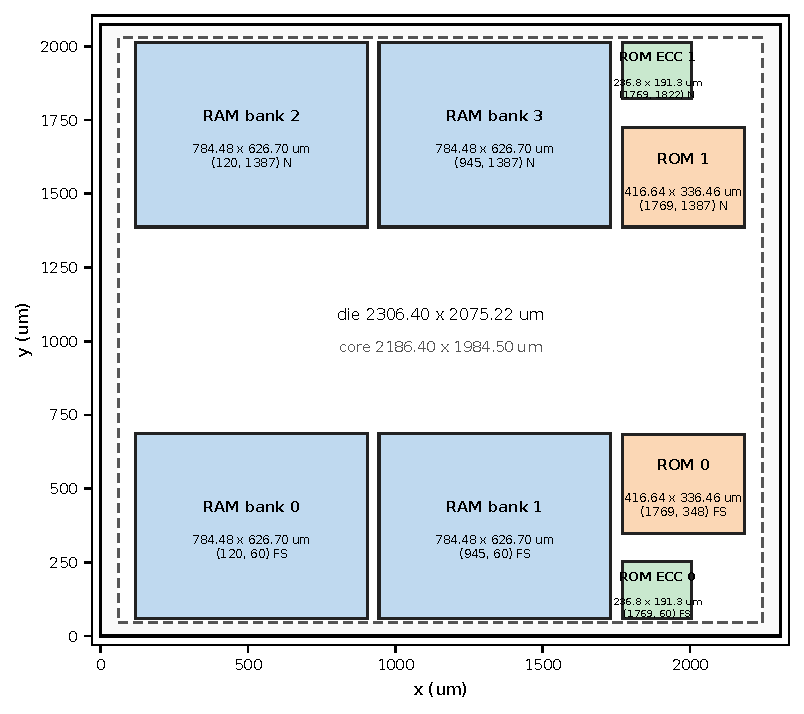
\includegraphics[width=\linewidth]{figures/floorplan_macros.pdf}
  \caption[Floorplan and the eight vendor macros]{The die outline, the
  core area and the eight vendor SRAM macros with their names, sizes and
  coordinates, drawn from the sign-off run's own DEF
  (\code{thesis/figures/make\_layout\_figures.py}). Four
  \code{RM\_IHPSG13\_1P\_2048x64} macros carry the RAM, two
  \code{1024x32} macros the boot ROM and two \code{512x16} macros the
  ROM's check bits. These are the parts the open decks cannot sign off
  (\dcite{12}{section 8}), which is why every geometric result in this
  work is reported as inside the macro hierarchy or outside it rather
  than as a total.}
  \label{fig:intro-macros}
\end{figure}

The third reason is also where the project's largest external blocker
lives, and \Cref{fig:intro-macros} is the picture of it. The macros the
open PDK ships cannot be signed off by the open decks at the pinned PDK
version. A trial harden containing one of them completed every flow
stage and ended with 1{,}106{,}478 Magic DRC error boxes, 2{,}316
KLayout DRC errors and 359 Netgen LVS errors --- and every one of the
Magic boxes, and every KLayout item, was \emph{inside the macro's own
footprint}, with the standard-cell area, the power grid and the routing
clean (\dcite{12}{section 7.5}). That Magic figure is a count of error
boxes and not of distinct violations: the flow's own report prints
``Should be divided by 3 or 4'' beneath the total, which puts the
distinct count at roughly 277{,}000--369{,}000 (\textbf{[estimate]}, the
report gives a range and not a divisor), and \dcite{12}{section 7.5}
quotes the raw box count everywhere with that caveat attached. The
conclusion does not depend on which end of the range is right: the
smallest reading is still hundreds of thousands of violations against a
required zero, and \dcite{12}{section 8} recorded a NO-GO for this PDK
version thirteen days before the gate that asked for it (\code{ROADMAP.md}
section 1). Two of the LVS
causes were diagnosed in that document --- hierarchy names that disagree
between the CDL and the extracted layout, so Netgen flattens the macro,
and bus index delimiters that disagree between angle brackets and square
brackets, so none of the macro's 188 bus pins match --- and the LVS half
is an open upstream issue.

That is why the geometric results on the eight-macro layout are stated
the way they are. On the \code{s83romecc5} layout, Netgen reports
\code{Circuits match uniquely} with all seven LVS counters at zero
(deck run \code{s83lvsbb2}), read
for exactly what it is: the vendor macro is a black box on both sides,
so the match signs off the connectivity \emph{into} the macros' pins and
says nothing about their internals. The KLayout deck declares 173 rule
categories in 47 groups and three fire, for 11{,}048 markers over 204
distinct cells --- 6{,}584 distinct shapes, because two of the three
rules are evaluated over the same derived layer and report an identical
set --- of which zero are outside the vendor macro hierarchy. The
abstracted Magic run reports 170 error boxes on \code{s83romecc5},
20 inside a macro
footprint and 150 outside, and every one of the 150 lies within
\qty{0.500}{\micro\metre} of a macro edge, none in open routing area,
because a LEF obstruction blanket is one shape more than
\qty{10}{\micro\metre} wide and ordinary routing beside it violates
wide-metal spacing rules that the macro's real geometry would not
(\dcite{67}{section 11}). \code{README.md} summarises the run with 182
Magic boxes and 162 outside, which reads like a contradiction and is
not one: 182 and 162 are run \code{s83ant}, the same layout with its
two antenna violations repaired, and the 60 diodes that repair inserted
moved routing inside the same halo --- 20 inside a footprint in both,
all 162 still within the same half micron, and the KLayout figures
identical marker for marker (\dcite{67}{section 11}). That is the shape
\Cref{sec:intro-rules} is about, and it had to be applied to this
chapter's own reading of its sources before it could be written down:
two correct statements about two different inputs, quoted without
saying which.

\section{Two parts: a frozen pilot and a system around it}
\label{sec:intro-two-parts}

The work is deliberately split in two, and the strategy is stated in
\code{ROADMAP.md} section 1: silicon-prove the PDK, the flow, a slice of
the inference fabric and the hardening demonstrators on a cheap shuttle
run before committing a full SoC.

\textbf{The pilot} is \code{tt\_um\_melihakbulut\_nssoc}, a
$6\times2$ = 12-tile design on the TTIHP26b shuttle, die area
\code{0 0 1289.28 313.74}\,\si{\micro\metre}, frozen at commit
\code{b6738e5} (\dcite{34}{section 1}). Its sign-off run closes setup at
every corner --- the slow corner at \qty{+1.2262}{\nano\second}, quoted
here to four decimals from a metric that carries more digits
(\code{+1.226180081066267}) --- with hold at
\qty{+0.1029}{\nano\second}, 33{,}564 instances at 48.7516\,\%
utilisation, and zeros for Magic DRC, LVS, detailed-route DRC, antenna
nets and pins, and total negative slack at all three corners, under a
5\,\% derate written into the flow's own constraint file
(\dcite{34}{section 3.3}). The Tiny Tapeout precheck passes 10 of 10
(\dcite{34}{section 7}). Its measured upset behaviour is a campaign of
378 injections classified against the golden model: 97 masked
(25.7\,\%), 193 corrected (51.1\,\%), 82 detected (21.7\,\%), 6 silent
data corruptions (1.6\,\%), 0 hangs, in 445.7\,s
(\dcite{64}{section 3.1}). At gate level, 370 of 370 comparable
injections classify identically to RTL (\dcite{32}{section 5.1}, quoted
by \code{README.md}).

The point of \code{docs/34} is not the numbers but the pinning: it answers
one question --- \emph{is what I am submitting the thing that was
verified?} --- and answers it so the answer can be checked by running
commands~\cite{lamb2022}. Ten RTL blobs by git hash, the submission tree
by a 31-file manifest whose own SHA-256 is recorded, six flow configurations pinned
by hash inside their own generator, and the built netlist, powered
netlist and DEF bit-identical across four independently configured
hardens of two configurations on two dates
(\code{docs/34} sections 2.1, 3.1, 3.2, 4 and 5.1). The GDS files differ
between those runs and that is expected, because GDS carries an embedded
generation timestamp: the GDS hash is a provenance record and not an
equality criterion, and the geometric equality is established by the
decks instead (\dcite{34}{section 3.2}).

What remains on the pilot is not engineering. The shuttle closes
2026-09-21 at 20:00 UTC, and the slot costs EUR~955 --- twelve tiles
at EUR~70 is EUR~840, plus a EUR~300 devkit subsidised to
EUR~100 while any of the subsidised boards remain, plus EUR~15 of
shipping (\code{docs/37} section 5 items 1 and 2, with the price table
both were read from in that document's section 1). Both the date and the price are
owner-side facts read from the vendor's own published records on
2026-08-31, and the close carries a time the project's earlier documents
did not record: 20:00 UTC, not local midnight (\dcite{37}{section 1}).
Buying the slot is the one item in \code{ROADMAP.md} section 4 that a
person must still do.

\textbf{The system-on-chip} under \code{hw/soc} is everything else. It
was begun after the pilot froze, it instantiates the frozen pilot rather
than copying it --- \code{hw/rtl/pilot\_top.v} inside \code{soc\_top.v},
reached over the same four serial pins the die will have --- and a
program running on Ibex out of the boot ROM configures it, loads its
weights, feeds it a six-frame event stream and reads the spikes back
against an answer the golden model computed at build time: 27 checks,
fail mask 0 (\code{docs/51}). The transport is serial because that is what
the die has, which costs 176 clock cycles per register access
(\dcite{53}{section 4.1}) and buys exactly one implementation of the
die's host protocol, the one in the system's own regression.

The freeze rule is what keeps the two apart. \dcite{34}{section 9}
states what does and does not void it: documents, tests and analysis
over existing run trees do not; any non-comment change to
\code{hw/rtl}, to the submission sources or to a pinned configuration
forces a full re-harden and a gate-level re-run. That rule has been
exercised twice --- once when two checkers were bound to all corners,
which forced a re-harden that reproduced the superseded runs on 196 of
196 and 194 of 194 metrics with the netlist bit-identical, and once when
the licensing decision added SPDX headers to every file in
\code{hw/rtl}, where all ten blobs moved and the netlist did not
(\code{docs/34} sections 1, 2.1 and 3.3). Both times the record was amended in
place with every superseded hash retained, because a freeze record that
can only be checked against \emph{now} is not a freeze record.

\section{Where the work is published}
\label{sec:intro-publication}

\begin{sloppypar}
The development repository is private and the published tree is a
generated mirror of it. \dcite{78}{section 1} takes that decision and
records what it costs: \code{scripts/gen\_public\_mirror.py} writes the
published subset into a directory and makes one commit naming the source
revision, it does not push and it does not create a repository, so
publication stays an act of the owner. The alternative --- making the
development repository public --- was declined for one honest reason:
three hundred-odd commit messages written over three weeks have not been
audited, and one missed message is not recoverable after a push
(\dcite{78}{section 1.1}). The mirror's cost is stated in its own
\code{README.md} rather than left for a reader to notice: you cannot see
how the design got here from the published repository, only where it
arrived. What makes that cost bearable is the corpus, which records the
withdrawn claims and the re-attributed measurements that a commit log
would not hold --- the history is published, it is just not in
\code{git log}.
\end{sloppypar}

\begin{sloppypar}
Three licences apply, one per kind of thing, decided in \code{docs/14} and
signed on 2026-09-09 (\dcite{14}{section 11}): CERN-OHL-W-2.0 for RTL,
testbenches, constraints, formal jobs and flow configuration;
Apache-2.0 for generators, golden models, harnesses, flow drivers,
analysis and CI; CC-BY-4.0 for the documents in \code{docs/} and the
measurement data. The reasoning is in \code{docs/14} sections 6.1--6.3 and
the load-bearing part of it is that the outbound choice was
\emph{unconstrained}: every inbound licence that touches a tracked file
is permissive, because third-party trees are fetched into gitignored
directories rather than vendored, so inbound obligations attach in only
two tracked places --- the Apache-2.0 Tiny Tapeout template scaffolding
under \code{tt/}, and two corrected copies of riscv-formal's own
instruction models, which carry upstream's ISC notice inline
(\code{docs/14} sections 2.1, 2.2 and 5.0). The reciprocal licence for
hardware was chosen against the permissive one for a stated reason:
the project's claimed differentiator is auditability, and a licence that
lets a derivative be closed undercuts the claim
(\dcite{14}{section 6.1}).
\end{sloppypar}

Three things are held back from the mirror, all commercial and none of
them technical: one section of the positioning document, the funding and
shuttle document, and the drafted text of an unsubmitted application.
Nothing technical is held --- no negative result, no withdrawn claim, no
measurement, no failing check --- and \dcite{78}{section 2} states why
that is a condition rather than a courtesy: a record that publishes only
what worked is a brochure. Each held file is replaced by a stub that
keeps the filename and says what was held, so that the corpus's own
cross-reference test still passes in the generated tree, which it does:
90 of 90 when that section was written (\dcite{78}{section 2.1}), and 95
by the time \dcite{78}{section 7} re-ran it a day later, because it is a
count of documents and not of findings. The mirror was first published on
2026-09-10 at 518 files from source revision \code{93757c9}, and
republished on 2026-09-11 at 529 files from \code{26f4494}
(\code{docs/78} sections 5 and 7).

\section{The rules this work holds itself to}
\label{sec:intro-rules}

A reader who takes nothing else from this chapter should take these
four. Each exists because the project broke it once and wrote down what
that cost.

\textbf{A superseded measurement is reported as superseded, with its
date, and is not rewritten.} This is \dcite{64}{section 2}'s method: the
original sentence stays where it was, struck through where a short
phrase is wrong or left whole and followed by a dated note, and the note
says what the value is now, why the old one was written, and which file
settles it. The document that established it was reconciling seven
figures the corpus stated two ways, and its first verdict is the reason
the rule is worth keeping: \emph{none} of the seven was a transcription
error. Every disagreement was two correct statements about two different
inputs --- an earlier run, a different source list, a different content
--- quoted without saying so (\dcite{64}{section 1}). The pilot's
fault-injection campaign is the clearest case: 335, 366 and 378 are all
real logs of the same file at three commits, and the history of that one
file settles which is the campaign of record without making the other
two wrong (\dcite{64}{section 3.1}). Where this document reports a
figure that a later measurement has moved, it reports both and says
which is which; where two documents in the repository still disagree, as
with the Magic box count in \Cref{sec:intro-pdk}, it says so and cites
both.

\textbf{No clock frequency is published for this design.}
\dcite{53}{section 9.2} refuses it in three ranked reasons. The first is
that the only available number is the frequency a layout happened to
reach, and a requirement written in the units of the answer is not a
requirement --- the derived requirement in that document is not a
frequency at all, it is a count of serial frames per second, and at the
geometry that exists the fabric caps that count long before the clock
does (\dcite{53}{section 6.5}). The second is \dcite{05}{section 4}
rule 5: any figure published externally must be traceable to measurement
or clearly labelled a design target, and the available figure is
neither, because it is the derived maximum frequency of a run that fails
setup on 2{,}003 endpoints, fails maximum slew at the slow corner and
fails maximum capacitance at all three. Half of that second reason has
since been superseded and the half that governs has not: the same
sentence in \dcite{53}{section 9.2} also said the layout had never seen
Magic DRC, KLayout DRC or Netgen LVS, and all four deck families have
run on \code{soc\_top}'s own geometry since 2026-09-11
(\code{README.md}, citing \code{docs/77} and \code{docs/79}); the slew
and capacitance failures are unchanged, and they are the half the rule
now rests on. The third reason is that two parts in
one project would carry two clocks and one of them is being fabricated,
and a reader offered both would ask which one the project's clock is.
What may be said instead is the stronger claim anyway: the mission
profiles have been sized, three of four are met with two to five orders
of magnitude of margin, and the fourth is a power requirement the design
does not meet with the mechanism named (\dcite{53}{section 9.4}).

\textbf{\textsc{timeout}, \textsc{killed} and \textsc{error} are three
different words.} \dcite{63}{section 16} spends thirty lines on the
distinction after a formal job was reported as a timeout and its own log
said otherwise: the job had been sent a signal from outside the run at
1\,h\,41\,m and the tool recorded \code{DONE (ERROR, rc=16)}, while no
timeout had been configured for it to reach. The reading each word
licenses is different. \textsc{timeout} means a bound was set, the job
reached it, and the measurement is complete --- \emph{this engine did
not close in that much time} --- and the jobs entitled to that word
wrote \code{rc=124} into their wall-time files, which is the
\code{timeout} utility saying it sent the signal itself. An error from
an outside kill means no bound was set and no measurement was completed,
and calling it a timeout would silently promote an interrupted run into
a finished experiment. The corpus has made that mistake in both
directions, and the fix is the same either way: read the runner's return
code before choosing the noun. The general form --- ``nothing came''
and ``I arrived late'' are not the same result --- is applied to a
testbench monitor in \dcite{81}{section 4.1}, which attributes the rule
to \code{docs/64} where the passage itself is in \code{docs/63}; both are
cited here because they disagree about the citation and not about the
rule.

\begin{sloppypar}
\textbf{A check must test the property, not the name.} The sharpest
statement of this is \dcite{78}{section 3}, and it is sharp because both
of its instances were in the project's own instruments rather than in
the design. The licence checker searched the first 4{,}000 characters of
a file for an identifier string in any context, so it read its own
docstring as its own licence header and reported zero missing while
carrying no header at all; it now counts a tag only on a comment line in
the first twelve lines, which is where a header is and where prose about
headers is not. The mirror generator carried a guard meant to refuse to
run if a workflow file no longer contained a sentence it rewrites ---
written as ``if the file is in the set'', so when the file was
\emph{deleted} the guard did not fire, it was skipped, and the generator
wrote 511 files as though nothing were owed. \dcite{78}{section 3.2}
records the conclusion in one line: a check that cannot fail when the
thing it checks is absent is not a check. That was the third instance of
the shape in this repository's own instruments and the first found in a
guard written to prevent it. The question is never ``did the check
pass'', it is ``what could the check have seen''. The corresponding rule
when a check is found to be narrow is \dcite{50}{section 8.1}'s:
\emph{extend, do not relax}.
\end{sloppypar}

Underneath all four sits a labelling convention used in every document
and carried into this one. \textbf{[fact]} means measured in this
environment or read out of a file; \textbf{[estimate]} means derived or
judged; \textbf{[planned]} means an intention with a date attached and
nothing behind it yet (\code{docs/00-index}, and the same three words at
the head of most documents in the corpus). Where a source marks a
statement with one of these, this document carries the mark rather than
flattening it.

\section{What this document is}
\label{sec:intro-status}

This is a record of measurements taken with open tools on a design that
exists in register-transfer and layout form. It is not a qualification
report and nothing in it should be read as one.

Concretely: there is no beam test, no lot, no screening and no
qualification body~\cite{ecss60_15c}; the fault-injection results are
simulated single-bit upsets, not measured event rates~\cite{nijsink2026};
the timing, power and area figures are pre-silicon flow results on layouts that are explicitly named where they
fail; and the memory macros the design depends on cannot be signed off
by the open decks at the pinned PDK version, so the die that carries
them cannot be either (\dcite{67}{section 11}). The claims this work
does make are of a different kind --- that a given mechanism is present
in the shipped netlist rather than only in the source, that a given
property holds over all reachable states, that a given campaign
classified a given number of injections a given way, that a given deck
found a given number of markers in a given place --- and each of them is
quoted here against the document that measured it, which in turn names
the command and the run tree it was read from.

\section{Road map}
\label{sec:intro-roadmap}

The remaining chapters are organised by what they measure rather than by
the order in which the work happened.

\textbf{The architecture chapter} describes the system as built: the
bus, the memory map frozen as a single generated source, the interrupt
and timing subsystem, the watchdog and its escalation ladder, the
peripherals, and the boot flow that initialises every word of an
error-correcting RAM before anything reads it --- because a memory whose
rows carry check bits powers up with an uncorrectable word everywhere,
not a zero. Its sources are \code{docs/38} through \code{docs/41},
\code{docs/65}, \code{docs/66} and \code{docs/68}.

\textbf{The accelerator chapter} describes the event-driven inference
engine, the register map generated from a single source, the serial
transport to it and what that transport costs, drawing on \code{docs/02},
\code{docs/10}, \code{docs/51} and \code{docs/53}.

\textbf{The hardening chapter} prices every protection mechanism
separately, because the project's discipline is that nothing is
protected before it is measured and every protection reports what it
cost: triple-modular redundancy on the state that cannot recover, SECDED
on the memories and the architectural register file, a scrub engine, and
fault counters an operator can read. Its sources are \code{docs/43},
\code{docs/44}, \code{docs/55}--\code{docs/58}, \code{docs/67} and \code{docs/69}.

\textbf{The verification chapter} covers the five layers and what each
can and cannot see: the cocotb regressions, the \emph{guards} that read
the tree without simulating it, the SymbiYosys property sets, the
riscv-formal bring-up against the ISA, and the seeded fault-injection
campaigns at register-transfer and gate level --- every one of them
judged against the bit-exact golden models that are the specification
(\code{docs/09}, \code{docs/11}, \code{docs/16}, \code{docs/32}, \code{docs/42},
\code{docs/52}, \code{docs/63}, \code{docs/74}, \code{docs/82}).

\textbf{The physical chapter} takes the design through the flow: the
floorplan and the decision behind it, the macro placement, synthesis,
place and route, the geometric decks and their macro-scoped results, and
the reproducibility record (\code{docs/12}, \code{docs/45}, \code{docs/47},
\code{docs/48}, \code{docs/59}, \code{docs/61}, \code{docs/71}, \code{docs/77},
\code{docs/79}). The layout figures introduced here are read in detail
there.

\textbf{The results chapter} puts the measurements side by side: what
closes, what does not, what each mechanism cost in area and in slack,
and what the power figures say once real switching activity is annotated
(\code{docs/57}, \code{docs/60}, \code{docs/76}, \code{docs/77}).

\textbf{The concluding chapter} states what remains open, in the terms
the record uses: the upstream macro blocker, the unmet idle-power
requirement, the serial transport that \dcite{53}{section 9.3} ranks
above timing, the provenance question of \Cref{sec:intro-not}, and the
one measurement nothing here substitutes for, which is silicon.
